\documentclass[aspectratio=169]{beamer}



\mode<presentation>
{
 \usetheme[reversetitle,notitle,noauthor]{Wien} 
%  \usetheme[noauthor]{Wien} 
}       
  
\usepackage{url}
\usepackage{graphicx}
\graphicspath{{./}{./Figures/}}  

\usepackage{appendixnumberbeamer} 

% To avoid a warning from the hyperref package:
\pdfstringdefDisableCommands{%
  \def\translate{}%
}

% To make sure, that the footnote is placed above and outside the
% footline (but it only works for one footnote per frame):
% 
% \addtobeamertemplate{footnote}{}{\vspace{4ex}}

%%%%%%%%%%%%%%%%%%%%%%%%%%%%%%%%%%%%%%%%%%%%%%%%%%%%%%%%%%%%%%%%%%%%%%%%%%%%% 
%%%%%%%%%%%%%%%%%%%%%%%%%%%%%%%%%%%%%%%%%%%%%%%%%%%%%%%%%%%%%%%%%%%%%%%%%%%%%
\title[Graphen-Spektren]{Graphen-Spektren}


\subtitle{Bachelorarbeit aus Diskreter Mathematik}

\author[R. Weiss]{Richard Weiss}

\institute[TU Wien]{TU Wien, Vienna, Austria}
   
\date{12. April 2021}

% Hier befinden sich Pakete, die wir beinahe immer benutzen ...

\usepackage[utf8]{inputenc}

% Sprach-Paket:
\usepackage[ngerman]{babel}

% damit's nicht so, wie beim Grill aussieht:
\usepackage{fullpage}

% Mathematik:
\usepackage{amsmath, amssymb, amsfonts, amsthm}
\usepackage{bbm}
\usepackage{mathtools, mathdots}

% Makros mit mehereren Default-Argumenten:
\usepackage{twoopt}

% Anführungszeichen (Makro \Quote{}):
\usepackage{babel}

% if's für Makros:
\usepackage{xifthen}
\usepackage{etoolbox}

% tikz ist kein Zeichenprogramm (doch!):
\usepackage{tikz}

% bessere Aufzählungen:
\usepackage{enumitem}

% (bessere) Umgebung für Bilder:
\usepackage{graphicx, subfig, float}

% Umgebung für Code:
\usepackage{listings}

% Farben:
\usepackage{xcolor}

% Umgebung für "plain text":
\usepackage{verbatim}

% Umgebung für mehrerer Spalten:
\usepackage{multicol}

% "nette" Brüche
\usepackage{nicefrac}

% Spaltentypen verschiedener Dicke
\usepackage{tabularx}
\usepackage{makecell}

% Für Vektoren
\usepackage{esvect}

% (Web-)Links
\usepackage{hyperref}

% Zitieren & Literatur-Verzeichnis
\usepackage[style = authoryear]{biblatex}
\usepackage{csquotes}

% so ähnlich wie mathbb
%\usepackage{mathds}

% Keine Ahnung, was das macht ...
\usepackage{booktabs}
\usepackage{ngerman}
\usepackage{placeins}

% special letters:

\newcommand{\N}{\mathbb{N}}
\newcommand{\Z}{\mathbb{Z}}
\newcommand{\Q}{\mathbb{Q}}
\newcommand{\R}{\mathbb{R}}
\newcommand{\C}{\mathbb{C}}
\newcommand{\K}{\mathbb{K}}
\newcommand{\T}{\mathbb{T}}
\newcommand{\E}{\mathbb{E}}
\newcommand{\V}{\mathbb{V}}
\renewcommand{\S}{\mathbb{S}}
\renewcommand{\P}{\mathbb{P}}
\newcommand{\1}{\mathbbm{1}}

% quantors:

\newcommand{\Forall}{\forall \,}
\newcommand{\Exists}{\exists \,}
\newcommand{\ExistsOnlyOne}{\exists! \,}
\newcommand{\nExists}{\nexists \,}
\newcommand{\ForAlmostAll}{\forall^\infty \,}

% MISC symbols:

\newcommand{\landau}{{\scriptstyle \mathcal{O}}}
\newcommand{\Landau}{\mathcal{O}}


\newcommand{\eps}{\mathrm{eps}}

% graphics in a box:

\newcommandtwoopt
{\includegraphicsboxed}[3][][]
{
  \begin{figure}[!h]
    \begin{boxedin}
      \ifthenelse{\isempty{#1}}
      {
        \begin{center}
          \includegraphics[width = 0.75 \textwidth]{#3}
          \label{fig:#2}
        \end{center}
      }{
        \begin{center}
          \includegraphics[width = 0.75 \textwidth]{#3}
          \caption{#1}
          \label{fig:#2}
        \end{center}
      }
    \end{boxedin}
  \end{figure}
}

% braces:

\newcommand{\pbraces}[1]{{\left  ( #1 \right  )}}
\newcommand{\bbraces}[1]{{\left  [ #1 \right  ]}}
\newcommand{\Bbraces}[1]{{\left \{ #1 \right \}}}
\newcommand{\vbraces}[1]{{\left  | #1 \right  |}}
\newcommand{\Vbraces}[1]{{\left \| #1 \right \|}}
\newcommand{\abraces}[1]{{\left \langle #1 \right \rangle}}
\newcommand{\round}[1]{\bbraces{#1}}

\newcommand
{\floorbraces}[1]
{{\left \lfloor #1 \right \rfloor}}

\newcommand
{\ceilbraces} [1]
{{\left \lceil  #1 \right \rceil }}

% special functions:

\newcommand{\norm}  [2][]{\Vbraces{#2}_{#1}}
\newcommand{\diam}  [2][]{\mathrm{diam}_{#1} \: #2}
\newcommand{\diag}  [1]{\mathrm{diag} \: #1}
\newcommand{\dist}  [1]{\mathrm{dist} \: #1}
\newcommand{\mean}  [1]{\mathrm{mean} \: #1}
\newcommand{\erf}   [1]{\mathrm{erf} \: #1}
\newcommand{\id}    [1]{\mathrm{id} \: #1}
\newcommand{\sgn}   [1]{\mathrm{sgn} \: #1}
\newcommand{\supp}  [1]{\mathrm{supp} \: #1}
\newcommand{\arsinh}[1]{\mathrm{arsinh} \: #1}
\newcommand{\arcosh}[1]{\mathrm{arcosh} \: #1}
\newcommand{\artanh}[1]{\mathrm{artanh} \: #1}
\newcommand{\card}  [1]{\mathrm{card} \: #1}
\newcommand{\Span}  [1]{\mathrm{span} \: #1}
\newcommand{\Aut}   [1]{\mathrm{Aut} \: #1}
\newcommand{\End}   [1]{\mathrm{End} \: #1}
\newcommand{\ggT}   [1]{\mathrm{ggT} \: #1}
\newcommand{\kgV}   [1]{\mathrm{kgV} \: #1}
\newcommand{\ord}   [1]{\mathrm{ord} \: #1}
\newcommand{\grad}  [1]{\mathrm{grad} \: #1}
\newcommand{\ran}   [1]{\mathrm{ran} \: #1}
\newcommand{\graph} [1]{\mathrm{graph} \: #1}
\newcommand{\Inv}   [1]{\mathrm{Inv} \: #1}
\newcommand{\pv}    [1]{\mathrm{pv} \: #1}
\newcommand{\GL}    [1]{\mathrm{GL} \: #1}
\newcommand{\Mod}{\mathrm{Mod} \:}
\newcommand{\Th}{\mathrm{Th} \:}
\newcommand{\Char}{\mathrm{char}}
\newcommand{\At}{\mathrm{At}}
\newcommand{\Ob}{\mathrm{Ob}}
\newcommand{\Hom}{\mathrm{Hom}}
\newcommand{\orthogonal}[3][]{#2 ~\bot_{#1}~ #3}
\newcommand{\Rang}{\mathrm{Rang}}
\newcommand{\NIL}{\mathrm{NIL}}
\newcommand{\Res}{\mathrm{Res}}
\newcommand{\lxor}{\dot \lor}
\newcommand{\Div}{\mathrm{div} \:}
\newcommand{\meas}{\mathrm{meas} \:}

% fractions:

\newcommand{\Frac}[2]{\frac{1}{#1} \pbraces{#2}}
\newcommand{\nfrac}[2]{\nicefrac{#1}{#2}}

% derivatives & integrals:

\newcommandtwoopt
{\Int}[4][][]
{\int_{#1}^{#2} #3 ~\mathrm{d} #4}

\newcommandtwoopt
{\derivative}[3][][]
{
  \frac
  {\mathrm{d}^{#1} #2}
  {\mathrm{d} #3^{#1}}
}

\newcommandtwoopt
{\pderivative}[3][][]
{
  \frac
  {\partial^{#1} #2}
  {\partial #3^{#1}}
}

\newcommand
{\primeprime}
{{\prime \prime}}

\newcommand
{\primeprimeprime}
{{\prime \prime \prime}}

% Text:

\newcommand{\Quote}[1]{\glqq #1\grqq{}}
\newcommand{\Text}[1]{{\text{#1}}}
\newcommand{\fastueberall}{\text{f.ü.}}
\newcommand{\fastsicher}{\text{f.s.}}

\theoremstyle{definition}

% unnumbered theorems
\newtheorem*{theorem*}    {Satz}
\newtheorem*{lemma*}      {Lemma}
\newtheorem*{corollary*}  {Korollar}
\newtheorem*{proposition*}{Proposition}
\newtheorem*{remark*}     {Bemerkung}
\newtheorem*{definition*} {Definition}
\newtheorem*{example*}    {Beispiel}
\newtheorem*{problem*}    {Problem}
\newtheorem*{algorithmus*}    {Algorithmus}
\newtheorem*{algorithmen*}    {Weiterführende Algorithmen}
\newtheorem*{anwendungen*}    {Anwendungen}

\renewcommand{\figurename}{Abbildung}
\renewcommand{\tablename} {Tabelle}


\begin{document}

\begin{frame}
  \titlepage
\end{frame}      

%%%%%%%%%%%%%%%%%%%%%%%%%%%%%%%%%%%%%%%%%%%%%%%%%%%%%%%%%%%%%%%%%%%%%%%%%%%%% 
%%%%%%%%%%%%%%%%%%%%%%%%%%%%%%%%%%%%%%%%%%%%%%%%%%%%%%%%%%%%%%%%%%%%%%%%%%%%%
%%%%%%%%%%%%%%%%%%%%%%%%%%%%%%%%%%%%%%%%%%%%%%%%%%%%%%%%%%%%%%%%%%%%%%%%%%%%%

\begin{frame}{Definitionen (1 / 5)}

  Man erinnere sich an die Definitionen der LVA \Quote{Diskrete und geometrische Algorithmen} WS 2020-21.

  \begin{definition*}[Mehr Graphen]
    Ungerichtete und gerichtete Graphen mit \textbf{Schleifen} haben auch Singletons bzw. Diagonal-Elemente der Knoten-Menge als Kanten. \\
    Bei \textbf{Multi-Graphen} ist die Kanten-Menge eine Multi-Menge.
  \end{definition*}

  Wir werden nur endliche Graphen brauchen.

\end{frame}


%%%%%%%%%%%%%%%%%%%%%%%%%%%%%%%%%%%%%%%%%%%%%%%%%%%%%%%
\begin{frame}{Mehr Graphen: Beispiele}

  \begin{figure}[H]
    \centering
    \subfloat[Ungerichteter Graph ohne Mehrfachkanten]
    {
        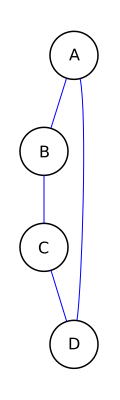
\includegraphics[height = 0.6 \textheight]{120px-Graph_ungerichtet.svg.png}
    }
    \hspace{1cm}
    \subfloat[Gerichteter Graph ohne Mehrfachkanten]
    {
        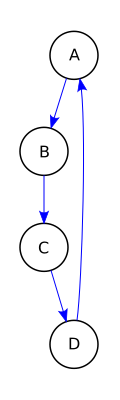
\includegraphics[height = 0.6 \textheight]{120px-Graph_gerichtet.svg.png}
    }
    \hspace{1cm}
    \subfloat[Ungerichteter Graph mit Mehrfachkanten]
    {
        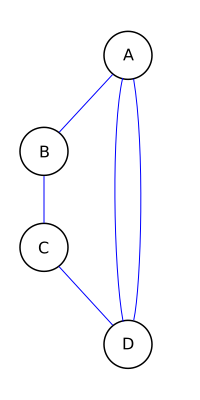
\includegraphics[height = 0.6 \textheight]{200px-Graph_ungerichtet_Mehrfachkanten.svg.png}
    }
    \hspace{1cm}
    \subfloat[Gerichteter Graph mit Mehrfachkanten]
    {
        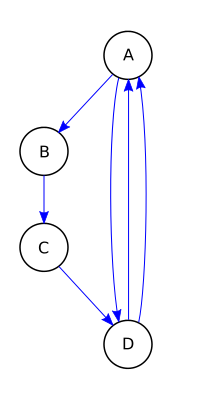
\includegraphics[height = 0.6 \textheight]{Graph_gerichtet_Mehrfachkanten.svg.png}
    }
    \hspace{0mm}
    % \caption
    % {
    %     Quelle:
    %     \url{https://de.wikipedia.org/wiki/Graph_(Graphentheorie)}
    % }
    \label{fig:2.1}
  \end{figure}

\end{frame}

%%%%%%%%%%%%%%%%%%%%%%%%%%%%%%%%%%%%%%%%%%%%%%%%%%%%%%%
\begin{frame}{Definitionen (2 / 5)}
  
  \begin{definition*}[Graphen-Matrizen]
    Sei $G = (V, E)$ ein (un)gerichteter (Mulit-)Graph mit oder ohne Schleifen und $V = \Bbraces{v_1, \dots, v_n}$ sowie $E = \Bbraces{e_1, \dots, e_m}$.
    Für $i, j = 1, \dots, n$ und $k = 1, \dots, m$ sei $a_{i, j}$ die Anzahl der Kanten von $v_i$ nach $v_j$, $d_i$ der (Eingangs-)Grad (ungerichtete Schleifen zählen doppelt) von $v_i$ und die Inzidenz zwischen $v_i$ und $e_k$

    \begin{align*}
      b_{i, k}
      =
      \begin{cases}
        1, & v_i \in e_k, \\
        0, & \text{sonst},
      \end{cases}
      \quad
      \text{bzw.}
      \quad
      b_{i, k}
      =
      \begin{cases}
        1, & \exists v \in V: e_k = (v_i, v), \\
       -1, & \exists v \in V: e_k = (v, v_i), \\
        0, & \text{sonst}.
      \end{cases}
    \end{align*}

    Wir nennen $\mathbf A := (a_{i, j})_{i,j=1}^n$ eine \textbf{Adjazenz-Matrix}, $\mathbf D := \diag(d_1, \dots, d_n)$ eine \textbf{Valenz-Matrix}, $\mathbf C := \mathbf D - \mathbf A$ eine \textbf{Laplace-Matrix} und $\mathbf B := (b_{i, k})_{i,k=1}^{n, m}$ eine \textbf{Inzidenz-Matrix} von $G$.

  \end{definition*}
  
\end{frame}

%%%%%%%%%%%%%%%%%%%%%%%%%%%%%%%%%%%%%%%%%%%%%%%%%%%%%%%
\begin{frame}{Graphen-Matrizen: Beispiele (0 / 4)}

  Betrachte die Graphen aus der vorherigen Abbildung.

  \begin{gather*}
    v_1 := A, v_2 := B, v_3 := C, v_4 := D, \\
    e_1 := \overline{A B},
    e_2 := \overline{B C},
    e_3 := \overline{C D},
    e_4 := \overline{D A}, \\
    e_{4, -1} := \overline{A D},
    e_{4, 1} := \overline{D A}^{(1)},
    e_{4, 2} := \overline{D A}^{(2)}
  \end{gather*}

  Die Mehrfachkanten seien dabei die letzteren $2$.
  Die Kanten seien lexikographisch bzgl. ihrer Indizes geordnet.

\end{frame}

%%%%%%%%%%%%%%%%%%%%%%%%%%%%%%%%%%%%%%%%%%%%%%%%%%%%%%%
\begin{frame}{Graphen-Matrizen: Beispiele (1 / 4)}

  \begin{multicols*}{2}
    
    \begin{figure}[H]
      \centering
      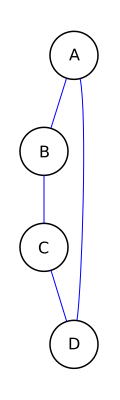
\includegraphics[height = 0.6 \textheight]{120px-Graph_ungerichtet.svg.png}
      \caption{Ungerichteter Graph ohne Mehrfachkanten}
    \end{figure}

    \begin{align*}
      \mathbf A
      & =
      \begin{pmatrix}
        0 & 1 & 0 & 1 \\
        1 & 0 & 1 & 0 \\
        0 & 1 & 0 & 1 \\
        1 & 0 & 1 & 0 \\
      \end{pmatrix}, \\
      \mathbf D
      & =
      \begin{pmatrix}
        2 & 0 & 0 & 0 \\
        0 & 2 & 0 & 0 \\
        0 & 0 & 2 & 0 \\
        0 & 0 & 0 & 2 \\
      \end{pmatrix}, \\
      \mathbf B
      & =
      \begin{pmatrix}
        1 & 0 & 0 & 1 \\
        1 & 1 & 0 & 0 \\
        0 & 1 & 1 & 0 \\
        0 & 0 & 1 & 1 \\
      \end{pmatrix}
    \end{align*}

  \end{multicols*}

\end{frame}

%%%%%%%%%%%%%%%%%%%%%%%%%%%%%%%%%%%%%%%%%%%%%%%%%%%%%%%
\begin{frame}{Graphen-Matrizen: Beispiele (4 / 4)}

  \begin{multicols*}{2}
    
    \begin{figure}[H]
      \centering
      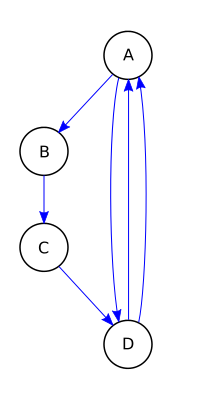
\includegraphics[height = 0.6 \textheight]{Graph_gerichtet_Mehrfachkanten.svg.png}
      \caption{Gerichteter Graph mit Mehrfachkanten}
    \end{figure}

    \begin{align*}
      \mathbf A
      & =
      \begin{pmatrix}
        0 & 1 & 0 & 1 \\
        0 & 0 & 1 & 0 \\
        0 & 0 & 0 & 1 \\
        2 & 0 & 0 & 0 \\
      \end{pmatrix}, \\
      \mathbf D
      & =
      \begin{pmatrix}
        2 & 0 & 0 & 0 \\
        0 & 1 & 0 & 0 \\
        0 & 0 & 1 & 0 \\
        0 & 0 & 0 & 2 \\
      \end{pmatrix}, \\
      \mathbf B
      & =
      \begin{pmatrix}
        0 & 0 & 0 & 1 & 1 & 0 \\
        1 & 0 & 0 & 0 & 0 & 0 \\
        0 & 1 & 0 & 0 & 0 & 0 \\
        0 & 0 & 1 & 0 & 0 & 1 \\
      \end{pmatrix}
    \end{align*}

  \end{multicols*}

\end{frame}

%%%%%%%%%%%%%%%%%%%%%%%%%%%%%%%%%%%%%%%%%%%%%%%%%%%%%%%
  
\begin{frame}{}
  
  \begin{remark*}
    Ein Graph $G$ ist durch eine seiner Adjazenz-Matrizen eindeutig bestimmt.
    Die Umkehrung gilt im Allgemeinen nur modulo Spalten- und Zeilen-Reihenfolge, d.h.

    \begin{align*}
      \forall \mathbf A_1, \mathbf A_2 \in \mathcal A(G):
        \exists \mathbf P ~\text{Permutations-Matrix}:
          \mathbf A_1 = \mathbf P^{-1} \mathbf A_2 \mathbf P,
    \end{align*}

    d.h. $G$ ist durch seine Klasse $\mathcal A(G)$ von Adjazenz-Matrizen eindeutig bestimmt.
    Adjazenz-Matrizen desselben Graphen haben dasselbe Spektrum.
    Dies rechtfertigt folgende Definition.
    
  \end{remark*}

\end{frame}

%%%%%%%%%%%%%%%%%%%%%%%%%%%%%%%%%%%%%%%%%%%%%%%%%%%%%%%
\begin{frame}{Definitionen (3 / 5)}
  
  \begin{definition*}[Gewöhnliches Spektrum \& Charakteristisches Polynom]
    
    Finde numerische Werte $\overline v \in \mathbb R$ für die Knoten $v \in V$ (als Variablen) eines Graphen $G = (V, E)$ mit $|V| = n$, sodass für alle Knoten $v$ das Verhältnis zwischen der Summe $\overline s_v$ der Werte der nach $v$ Knoten $w \to v$ (die über eine Kante nach $v$ führen) und $\overline v$ konstant ist, d.h.
  
    \begin{align*}
      \exists \lambda \in \mathbb C:
        \forall v \in V:
          \overline s_v = \sum_{w \to v} \overline w = \lambda \overline v.
    \end{align*}
  
    Sei $\mathbf A \in \mathcal A(G)$, dann können wir das umformulieren zu $\mathbf A \mathbf v = \lambda \mathbf v$. \\
    Eine notwendige und hinreichende Bedingung für die Existenz eines solchen $\mathbf v$ ist, dass $\lambda$ Nullstelle des \textbf{gewöhnlichen Charakteristischen Polynoms} $P_G(\mu) := \det(\mu \mathbf I_n - \mathbf A)$. \\
    $\lambda$ ist dann Teil des \textbf{gewöhnlichen Spektrums} $\sigma_P(G) := \sigma(\mathbf A)$ von $G$.

  \end{definition*}

\end{frame}

%%%%%%%%%%%%%%%%%%%%%%%%%%%%%%%%%%%%%%%%%%%%%%%%%%%%%%%
\begin{frame}{Zusammenfassung: \Quote{spektrale} Eigenschaften von Graphen}

  \begin{block}{}

    \begin{itemize}
      \item Graphen-Matrizen z.B. $\mathbf A$, $\mathbf D$, \dots,
      \item (Koeffizienten von) verschiedene(n) Charakteristische(n) Polynome(n) z.B. $P_G(\lambda)$, $Q_G(\lambda)$, \dots
      \item Graphen-Spektren z.B. $\sigma_P(G)$, $\sigma_Q(G)$, \dots
    \end{itemize}

  \end{block}

\end{frame}

%%%%%%%%%%%%%%%%%%%%%%%%%%%%%%%%%%%%%%%%%%%%%%%%%%%%%%%
\begin{frame}{Definitionen (4 / 5)}

  \begin{definition*}[Kanten-Graph]

    Der \textbf{Kanten-Graph} $L(G) = (V^\prime, E^\prime)$ eines ungerichteten Graphen $G = (V, E)$ hat als Knoten die Kanten von $G$ und diese sind adjazent, wenn sie als $G$-Kante einen gemeinsamen $G$-Knoten habend, d.h.

    \begin{align*}
      V^\prime = E,
      \quad
      E^\prime = \Bbraces{\Bbraces{e_1, e_2}: e_1, e_2 \in E, e_1 \cap e_2 \neq \emptyset}.
    \end{align*}

  \end{definition*}

  \begin{definition*}
    Die \textbf{direkte Summe} $G = G_1 \dotplus G_2$ der Graphen $G_1 = (V_1, E_1)$ und $G_2 = (V_2, E_2)$ mit $E_1 \cap E_2 = \emptyset$ ist $G = (V, E)$ mit $V = V_1 \cup V_2$ und $E = E_1 \cup E_2$.
  \end{definition*}

\end{frame}

%%%%%%%%%%%%%%%%%%%%%%%%%%%%%%%%%%%%%%%%%%%%%%%%%%%%%%%

\begin{frame}{Definitionen (5 / 5)}

  \begin{definition*}[NEPS]

    Seien $G_1 = (V_1, E_1), \dots, G_n = (V_n, E_n)$ Graphen. Deren \textbf{NEPS} (\Quote{Non-complete Extended $P$-Sum}) bzgl. $\mathcal B \subseteq \Bbraces{0, 1}^n \setminus \Bbraces{(0, \dots, 0)}$ sei der Graph $G$ mit folgender Knoten- bzw. Kanten-Menge.
  
    \begin{align*}
      V & := \prod_{i=1}^n V_i, \\
      E
      :=
      \{ &
        ((v_1, \dots, v_n), (w_1, \dots, w_n)) \in V^2:
        \exists (\beta_1, \dots, \beta_n) \in \mathcal B: \\ &
          \forall i = 1, \dots, n:
            (\beta_i = 1 \implies (v_i, w_i) \in E_i),
            (\beta_i = 0 \implies v_i = w_i)
      \}.
    \end{align*}

  \end{definition*}
  
  % \begin{definition*}[prominente NEPS]
  %   \begin{itemize}
  %     \item $\mathcal B = \Bbraces{(1, 1)}$ \dots $G = G_1 \times G_2$ \textbf{direktes Produkt}
  %     \item $\mathcal B = \Bbraces{(0, 1), (1, 0)}$ \dots $G = G_1 + G_2$ \textbf{Summe}
  %   \end{itemize}
  % \end{definition*}

\end{frame}

%%%%%%%%%%%%%%%%%%%%%%%%%%%%%%%%%%%%%%%%%%%%%%%%%%%%%%%
\begin{frame}{Wichtige Fragestellungen}

  \begin{block}{}

    \begin{itemize}

      \item Zusammenhänge zwischen (unter) verschiedenen \Quote{spektralen} Eigenschaften

      \item \Quote{spektrale} Eigenschaften \dots

      \begin{itemize}
        \item von prominenter Graphen (und deren Zusammenhänge),
        \item von Graphen durch Graphen-Operationen (vs. Graphen-Matrix-Operationen z.B. $+$, $\cdot$, $\det$, $\otimes$, \dots),
        \item (effiziente) Berechnung
        \item Zusammenhänge zum Graphen selbst (geometrische Eigenschaften) in beide Richtungen!
      \end{itemize}

    \end{itemize}

  \end{block}

\end{frame}

%%%%%%%%%%%%%%%%%%%%%%%%%%%%%%%%%%%%%%%%%%%%%%%%%%%%%%%
\begin{frame}{}

  \begin{block}{}

    {
      \centering
      \huge
      Ende des Crashkurses!
    }

  \end{block}

\end{frame}

\appendix

%%%%%%%%%%%%%%%%%%%%%%%%%%%%%%%%%%%%%%%%%%%%%%%%%%%%%%%
\begin{frame}{Aussicht auf Spezialisierung}

  Jedes chemische Molekül kann als \textbf{molekularer Graph} dargestellt werden:
  Die Ecken entsprechen Atomen und die Kanten deren Bindungen.
  Die $\pi$-Elektronen-Energie (Energie der Elektronen in $\pi$-Orbitalen) von Kohlen-Wasserstoffen entspricht der \dots
  
  \begin{definition*}[Energie eines Graphen]

    Sei $G$ ein Graph, dann lautet seine Energie

    \begin{align*}
      \mathcal E(G)
      :=
      \sum_{\lambda \in \sigma_P(G)} |\lambda|.
    \end{align*}

  \end{definition*}

\end{frame}

%%%%%%%%%%%%%%%%%%%%%%%%%%%%%%%%%%%%%%%%%%%%%%%%%%%%%%%
\begin{frame}{}
 
  % \begin{figure}[H]
  %   \centering
  %   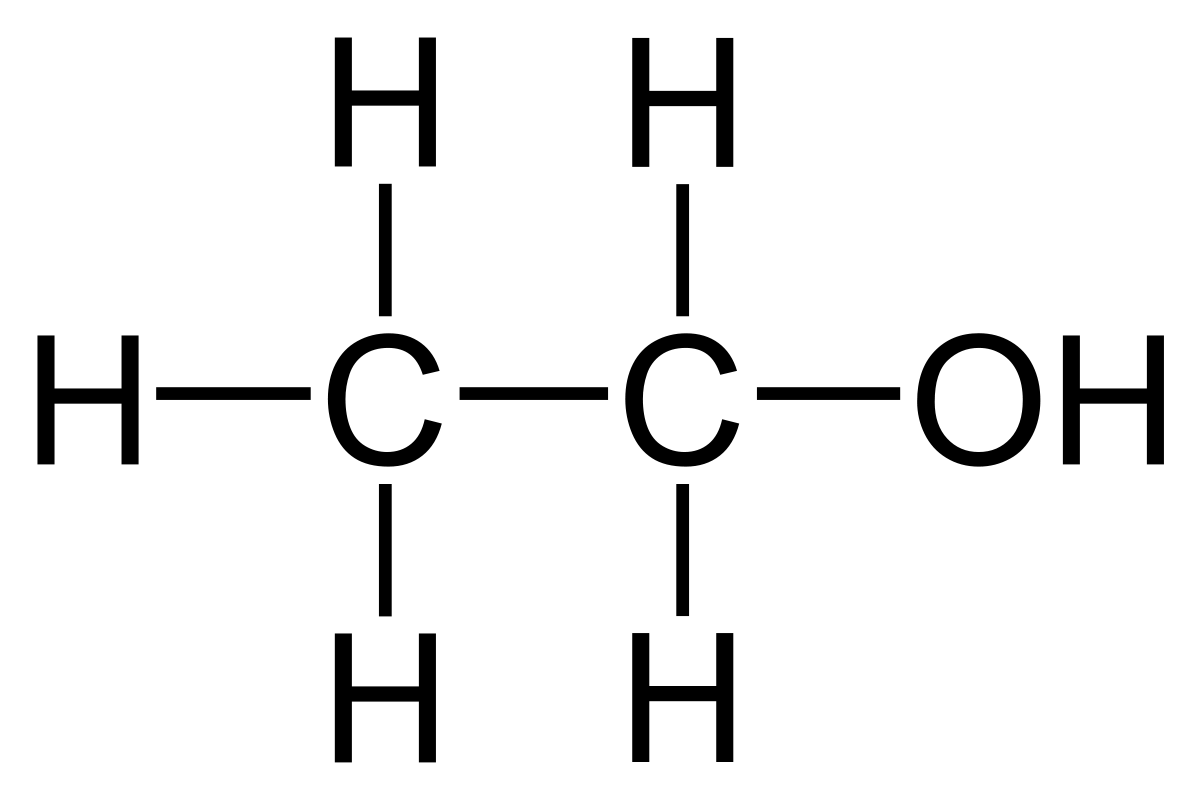
\includegraphics[width = 0.3 \textwidth]{1200px-Ethanol_Lewis.svg.png}
  %   \caption
  %   {
  %     Quelle:
  %     \href
  %     {https://de.wikipedia.org/wiki/Ethanol}
  %     {https://de.wikipedia.org/wiki/Ethanol}
  %   }
  % \end{figure}
  
  \begin{block}{}

    {
      \centering
      \huge
      To be continued ... am 7. Juni 2021.
    }

  \end{block}

\end{frame}

%%%%%%%%%%%%%%%%%%%%%%%%%%%%%%%%%%%%%%%%%%%%%%%%%%%%%%%%%%%%%%%%%%%%%%%%%%%%% 
%%%%%%%%%%%%%%%%%%%%%%%%%%%%%%%%%%%%%%%%%%%%%%%%%%%%%%%%%%%%%%%%%%%%%%%%%%%%%

\end{document}


%%% Local Variables:
%%% mode: latex
%%% TeX-master: t
%%% End:
